\documentclass{article}
\usepackage{hyperref}
\usepackage{tikz}
\usepackage{python}
\usepackage[%
    natbib=true,%
    backend=biber,%
    backref=true,%
    citestyle=authoryear-comp,%
    bibstyle=authoryear,%
    maxbibnames=24,%
    maxcitenames=2,%
]{biblatex}

\hypersetup{%
    bookmarks=true,
    colorlinks=true,
    pdfauthor={Luis Pedro Coelho},
    citecolor=pondgreen,
    urlcolor=toastedchilipowder,
    linkcolor=toastedchilipowder,
}
\let\code\texttt
\addbibresource{references.bib}
\addbibresource{readcube_export.bib}

\title{Jug: Software for Reproducible Computation In Python}
\author{Luis Pedro Coelho}

\begin{document}
\maketitle

\section*{Abstract}
As computational pipelines become a bigger part of science, it is important to
ensure that the results are reproducible, a concern which has come to the fore
in recent years. All developed software should be able to be run automatically
without any user intervention.

In addition to being valuable to the wider community, which may wish to
reproduce or extend a published analysis, reproducible research practices allow
for better control over the project by the original authors themselves. For
example, if necessary parameters to run a pipeline are kept separately from the
code that implements it, this leads to error-prone analysis and opens up the
possibility that, when the results are to be written up for publication, the
researcher will no longer be able to even completely describe the process that
led to them.

For large projects, the use of multiple computational cores (either in a
multi-core machine or distributed across a compute cluster) is necessary to
obtain results in a useful time frame. Furthermore, it is often the case that,
as the project evolves, it becomes necessary to save intermediate results while
down-stream analyses are designed (or re-designed) and implemented. Under many
frameworks, this causes having a single point of entry (often in the form of a
single script or a single main programme) for the computation becomes
increasingly difficult.

Jug is a software framework which solves all of these problems in a simple way.
Jug supports caching of intermediate results, distribution of computation as
tasks across a network.

Jug is written in pure Python, is completely cross-platform, and available as
free software under the liberal MIT license. Jug is available from
\url{http://github.com/luispedro/jug}.
\bigskip
\bigskip

\section{Introduction}
The value of reproducible research in computational fields has been recognized
in several areas
\citep{donoho2009reproducible,v2009reproducible,nordlie2009towards,fomel2015reproducible,leveque2012reproducible,dudley2010reproducible}.
Although some of the reports are still more forward looking rather than
descriptive of current practice, several implementations of reproducible papers
(or executable papers) have been proposed towards the goal of reproducing
published analyses.

These solutions do not necessarily scale to large problems, those that take
several days, months, or years of CPU time. For very large problems,
specialized solutions are needed~\citep{dean2008mapreduce,zaharia2010spark}.
There is a range of medium-sized problems that can be successfully tackled on a
computer cluster with a small number of nodes or even taking advantage of a
single multicore machine.

The typical ad hoc solution to this problem is to save intermediate files on
disk. A limitation of this approach is that often the design of the computation
itself takes several iterations as intermediate steps are improved. Thus, some
intermediate results need to be recomputed. This involves a large amount of
human management of the state of the computation, breaking it up into pieces,
and issuing jobs on the cluster.

Jug is a task-based framework for Python, which supports saving and sharing of
intermediate results and parallelisation on computer clusters (or multi-core
machines).

By allowing caching of results, where the caching depends explicitly on the
input parameters of that computation. Any change in the parameters immediately
triggers a recomputation of all dependent results. The basic model is similar
to the one of the venerable Unix tool Make, which has been used before for
implementing reproducible research pipelines~\citep{Schwab00makingscientific}.

However, unlike make, jug is written in Python, a general purpose programming
language which is widely used in scientific programming \citep{prabhu2011a}.  A
Task in Jug can consist of any Python function and its arguments. The task can
include running external commands and calling routines written in other
languages as Python has many tools to interface with the rest of the system
\citep{beazley1996swig,beazley2003automated,behnel2011cython}.

A Jugfile (the file which specifies which tasks need to be run---named by
analogy to the Makefiles of make) is a simple Python script with some added
notations (we will see the only a few, small, changes are needed to transform a
conventional Python script into a Jugfile).

\section{Design Choices}
\subsection{Task Based Architecture}

Jug is designed around tasks. A task is defined as a Python function and a set
of arguments, which may be Python values or the output of other tasks.

For example:

\begin{python}
from jug import Task

def count(imname):
    ...
    return value

def mean(args):
    return sum(args)/float(len(args))

images = glob('*.png')
counts = [Task(count, im) for im in images]
final = Task(mean, counts)
\end{python}

\begin{figure}
\begin{center}
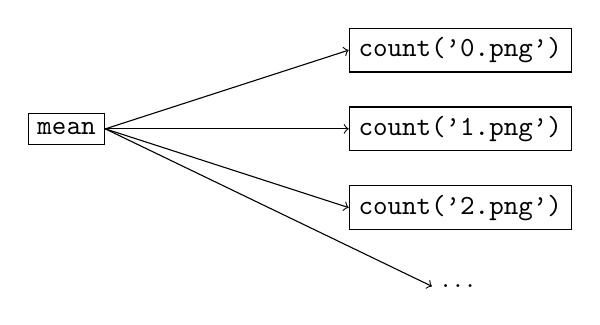
\begin{tikzpicture}
\node (mean) at (0,2) [draw] {\code{mean}};
\node (count0) at (5,3) [draw] {\code{count('0.png')}};
\node (count1) at (5,2) [draw] {\code{count('1.png')}};
\node (count2) at (5,1) [draw] {\code{count('2.png')}};
\node (countn) at (5,0) {\ldots};

\draw[->] (mean.east) -- (count0.west);
\draw[->] (mean.east) -- (count1.west);
\draw[->] (mean.east) -- (count2.west);
\draw[->] (mean.east) -- (countn.west);
\end{tikzpicture}

\end{center}
\caption{Simple Dependency Structure for Example in the Text. This assumes that
the directory had a collection of images names 0.png, 1.png,\ldots}
\label{fig:jug-deps}
\end{figure}

This code defines the task dependency structure represented in
Figure~\ref{fig:jug-deps}. As we can see, all of the \code{count} operations
can be run in parallel, while the \code{mean} operation must wait the result of
all of the other computation. The dependency structure is always a \textsc{dag}
(directed acyclic graph).

The code above has the construct \code{Task(f, args)} repeated several times.
Using the decorator \code{TaskGenerator} decorator this can be simplified to a
more natural syntax.

\begin{python}
from jug import TaskGenerator

@TaskGenerator
def count(imname):
    ...
    return value

@TaskGenerator
def mean(args):
    return sum(args)/float(len(args))

images = glob('*.png')
counts = map(count, images)
final = mean(counts)
\end{python}

As the reader can appreciate, this is identical to a traditional Python script,
except for the \code{@TaskGenerator} decorators. With a few limitations (which
unfortunately can give rise to complex error messages), scripts can be written
as if they were sequential Python scripts.

By default, jug looks for a file called \code{jugfile.py}, but any filename can
be used. Generically, we refer to the script being run as the Jugfile.

\subsection{Jug subcommands}

Jug is structured as a series of subcommands, the most important of which are
\emph{execute}, \emph{status}, and \emph{shell}.

Execution is the command used for running the tasks. It performs a more complex
version of the following pseudo-code:

\begin{python}
tasks = alltasks in topological sort order
while tasks:
    next = task.pop()
    if not next.has_run() and not next.is_running():
        while not next.can_run():
            wait a while
        with locked(next):
            next.run()
\end{python}

If run on a single processor, this will just run all of the tasks in order. It
is most interesting when it is run on multiple processors. Because of the lock
synchronisation, tasks can be run in parallel to take advantage of the multiple
cores.

The actual code is more complex than what is shown above, particularly to make
sure that the locking is performed correctly and that the waiting step
eventually times out (in order to handle the situation where another process is
hung).

\begin{figure}
\begin{verbatim}
$jug status images.py
Task name         Waiting      Ready   Finished    Running
----------------------------------------------------------
images.mean             1          0          0          0
images.count            0         20          0          0
..........................................................
Total:                  1         20          0          0
\end{verbatim}
\caption{Output of \code{jug status}. The \texttt{\$} sign shown is the command
line prompt, and the status subcommand was run. At this point, nothing has been
run. The output has been edited for space reasons (spacing columns were
removed).}
\label{fig:jug-status-output}
\end{figure}

The \texttt{status} subcommand prints out a summary of the status of all of the
tasks. Figure~\ref{fig:jug-status-output} shows the output of this command
using the example jugfile above. We assume that the jugfile was called
\code{images.py} on disk and that there were 20~images in the directory. We can
see that there are 20~tasks ready to run, while the \code{mean} task is still
waiting for the results of the other tasks.

\subsection{Backends}

A basic feature of jug is its ability to save and load results. Each task
\code{Task(f, args)} is represented by a hash of \code{f} and \code{args} in a
way that uniquely identifies it.

A jug backend must then support four basic operations:

\begin{description}
\item[save] Saving a Python object by its hash name.
\item[load] Loading a Python object by its hash name.
\item[lock] Creating a lock by hash name. Naturally, this lock must be created
atomically.
\item[release] Releasing the lock.
\end{description}

A few other operations, such as deletion and listing of names are also
supported.

The filesystem can support all of the above operations if the backend is coded
correctly to avoid race conditions. This is the default backend, identified
simply by a directory name. Inside this directory, files named by a hexadecimal
representation of their hashes. Objects are saved using Python's \code{pickle}
module with zlib compression. As a special case, \code{numpy} arrays
\citep{walt2011the} are saved to disk directly. This special case was
introduced as \code{numpy} arrays are a very common data type in scientific
programming and saving them directly allows for very fast saving and loading
(they are represented on disk as a header followed by the binary information
they contain).

Another backend currently included with jug is a redis backend. Redis a
name-key database system.\footnote{See the redis webpage, at
\href{http://redis.io}{redis.io}, for detailed information about redis.} Redis
is particularly recommended for the case where there are many small objects
being saved. In this case, keeping each as a separate file on disk would incur
a large space penalty, while redis keeps them all in the same file.

Finally, there is an in-memory backend. This was initially developed for
testing, but can be useful on its own.

\subsection{Asynchronous Function}

Parallelisation is achieved by running more than one jug process
simultaneously. All of the synchronisation is outsourced to the backend. As
long as all of the processes can access the backend, there is no need for them
to communicate directly. It can even be the case that processors start working
on tasks in mid-processing. This makes jug usable in batch-based computer
cluster environments, which are quite common in research institutions.

\subsection{Software Development With Jug}

The output of computation can be obtained from jug in three ways: (1) One can
write a task that writes the output to a file in the desired format. (2)
Outputs can be inspected interactively using the \emph{shell} subcommand. It is
expected that the first option will be used for the final version of the
computation, whilst the second one is most helpful during development. Finally,
(3) jug can be loaded as a library from a Python script and jug computation
outputs can serve as inputs for further computation. This can be performed from
inside a Jupyter notebook \citep{kluyver2016jupyter}.

The shell subcommand, invokes an Jupyter instance with all the objects in the
jugfile loaded. The Jupyter console is an enhanced interactive shell for Python
\citep{perez2007ipython}. A few functions are added to the namespace, in
particular, \code{value} can load the results of a task object if necessary.

\begin{figure}
\begin{center}
\begin{verbatim}
$jug shell images.py

Available jug functions:
    - value() : loads a specific object
    - load_all() : loads all objects


In [1]: value(final)
Out[1]: 7.5

In [2]: value(counts)
Out[2]: [7, 7, 7, 7, 7, ... 8, 8, 8, 8, 8, 8, 8, 8, 8]
\end{verbatim}
\end{center}
\caption{Interaction with \code{jug shell}. The \code{value} function loads and
returns the result from any task. The final line has been edited (marked with
\ldots) for presentation purposes.}
\label{fig:jug-shell-interaction}
\end{figure}

Figure~\ref{fig:jug-shell-interaction} shows a possible interaction session
with jug shell. While having to explicitly load all the results may be
bothersome, it is both much faster at start up and the user might not load more
than a few objects throughout their session. In some cases, loading all of the
objects simultaneously might even be impossible due to memory constraints.
Furthermore, this allows exploration of the task structure for debugging.

\subsection{Result Invalidation}

If a researcher improves an intermediate step in a pipeline (e.g., fixes a bug)
and wishes to obtain new results of the computation, then all outputs from that
step and downstream must be recomputed, but results from upstream and unrelated
processes can be reused. Formally, in the task DAG, affected tasks and their
descendants must be recomputed. Without tool support, this can be a very
error-prone operation: by not removing enough of the intermediate files, it was
easy to generate an irreproducible state where part of the computations were
made using one version of the code and part with another.

Therefore, jug adds support for result invalidation. When a results from a task
are invalidated, all tasks which (directly or indirectly) depend on them are
also invalidated.

It is still necessary to manually invalidate tasks. An alternative, would be to
take code which implements the task into account while computing the hash. This
would mark any results computed with this code as outdated if the code changed.
While this would add another layer of protection, it would still be possible to
make mistakes. If the function depended on other functions, especially if this
was done in a dynamic way, it could be hard to discover all dependencies (cf.\
sumatra, which does capture all dependencies that are necessary to run a
particular computation \citep{davison2012automated}). Additionally, even minute
refactoring of the code would lead to over eager recomputation. This could make
the developer wary of making improvements in their code, resulting in overall
worse code.

Therefore, as a design choice, jug asks the user to explicitly invalidate their
results, while supporting automatic dependency discovery. The recommendation is
still that the user run the full pipeline from start to finish once they are
satisfied with the state of the code and certainly before publication, but the
pipeline development stage can be more agile.

\section{Example}
This section presents an edited version of the code used in a previously
published study of computer vision techniques for bioimage
analysis~\cite{coelho2013determining}. The goal of this project was to
demonstrate that using local features, in particular speeded-up robust features
(henceforth, \textsc{surf}) improves over image-global features for
classification of microscope images.

To evaluate classification, the dataset is broken up into 10~pieces and each of
the pieces is held-out of the analysis and then used to evaluate analysis (the
final result is the average of all ten values). This is known as
cross-validation.

\begin{python}
from jug import TaskGenerator, CachedFunction
import mahotas as mh
from sklearn.cross_validation import KFold

def load():
    '''
    This function assumes that the images are stored in
    data/<dset> with filenames matching the pattern
    label-protein-([0-9]).tiff
    '''
    from os import listdir
    images = []
    base = './data/'
    for path in listdir(base):
        if not 'protein' in path: continue
        label = path.split('-')[0]
        # We only store paths and will load data on demand
        # This save memory.
        im = (base + path, label)
        images.append(im)
    return images


# TaskGenerator can be used with any function, including builtins:
jug_sum = TaskGenerator(sum)

@TaskGenerator
def computefeatures(im):
    im = mh.imread(im)
    return mh.features.haralick(im)

@TaskGenerator
def output(cmatrix, dset, fset):
    with open('results/cmatrix-'+dset+'-'+fset+'.txt', 'w') as output:
        output.write(cmatrix)
        output.write('\n')

@TaskGenerator
def train_test1(features, labels, train, test):
    from sklearn import linear_model
    from sklearn import metrics
    clf = linear_model.LogisticRegression()
    clf.fit(features[train], labels[train])
    preds = clf.predict(features[test])
    return metrics.confusion_matrix(labels[test], preds)


images = CachedFunction(load)
features = []
images = []
for im,label in images:
    labels.append(label)
    features.append(haralick(im))
cmats = []
for train,test in KFold(len(features), n_folds=10):
    cmats.append(
        train_test1(features, labels, train, test))
return jug_sum(cmats)
cmatrix = nfoldcrossvalidation(features, labels)
output(cmatrix, dset, fset)
\end{python}

Figure~\ref{fig:jug-deps-complex} shows the dependency structure of this
examples. The main feature is the fan-out/fan-in which is associated with
map-reduce frameworks.

\begin{figure}
\begin{center}
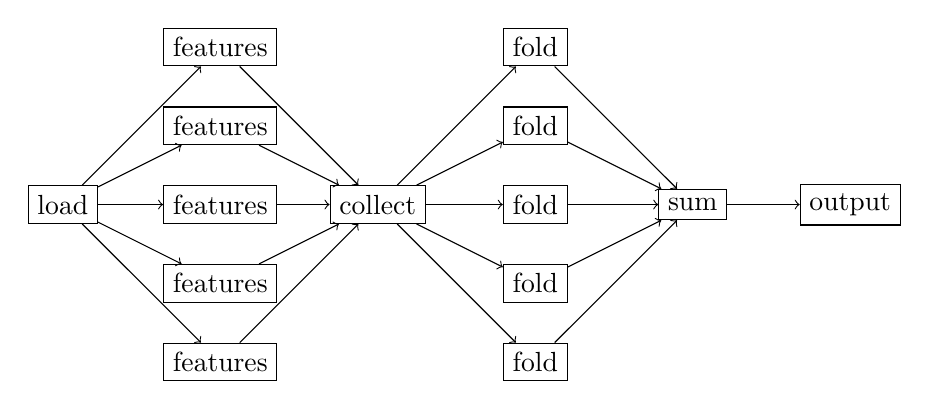
\begin{tikzpicture}
\node (load) at (0,0) [draw] {load};
\node (collect) at (4,0) [draw] {collect};
\node (sum) at (8,0) [draw] {sum};
\node (output) at (10,0) [draw] {output};

\path[->]
    (sum) edge (output);

\foreach \y in {-2,-1,0,1,2} {%
    \node (features\y) at (2,\y) [draw] {features};
    \path[->]
        (load) edge (features\y)
        (features\y) edge (collect);
}

\foreach \y in {-2,-1,0,1,2} {%
    \node (fold\y) at (6,\y) [draw] {fold};
    \path[->]
        (collect) edge (fold\y)
        (fold\y) edge (sum);
}
\end{tikzpicture}

\end{center}
\caption{Dependency Structure for second example in the Text. The
fan-out/fan-in structure is typical (it is an instance of the map-reduce
framework).}
\label{fig:jug-deps-complex}
\end{figure}

\section{Development of Jug}
Jug is available under the MIT software license, which grants the user right to
use, copy, and modify the code almost at will. It is developed using the git
version control tool, with the project being hosted on the github
platform.\footnote{The jug project is available at
\url{https://www.github.com/luispedro/jug}.} An open mailing-list provides
support and reported bugs are generally fixed within hours or days.

Jug includes a full test suite with continuous integration, which are best
practices \citep{wilson2014best} which can improve productivity
\citep{vasilescu2015quality}. There are no known bugs.

\section{Discussion}

\subsection{Similar Tools}

Several pipeline tools have been used (for a recent review, see the work of
\citet{leipzig2016a}). \citet{2007reproducible} proposed a system built on
top of Scons which shared superficially similar design. Scons, like Make, is a
build system. It supports spawning parallel jobs using multiple threads. In the
original use case, the tasks are delegated to other commands and the operating
system can take care of parallelism. If, however, the tasks are computationally
intensive in Python, contention for the global interpreter lock will limit the
amount of real parallelism.\footnote{In the most commonly used Python
interpreters, there is a lock that prevents more than one thread from
simultaneously executing interpreted code, although they can execute
non-interpreted code, as calling an external programme or certain external
libraries.} Ruffus is another Python-based solution which supports parallel
execution of pipelines \citep{goodstadt2010ruffus}. Using the Ruby programming
language, \citet{mishima2011} proposed Pwrake, which supports parallel
execution of bioinformatics workflows written (or accessible) in that language.
Snakemake~\citep{kster2012snakemakea} also improves over Make by providing more
complex rules and automatic interaction with a high performance compute
cluster. \citet{sadedin2012bpipe} proposed Bpipe, a tool based on a
domain-specific language around shell scripting. One large difference of Jug
compared to these tools is that Jug is tightly integrated with Python code.
Thus, while it lacks support for directly spawning processes like Make, it is
easier to call Python-based functions.

Also relevant is the \textsc{IncPy} implementation of a Python interpreter with
automatic persistent memoization~\cite{guo2010towards,guo2011using}
(unfortunately, no longer maintained). The advantages of that system apply to
Jug as well, with a few differences. Their system implements automatic
memoization, while, using Jug, the user needs to automatically annotate
functions to memoize using \texttt{TaskGenerator}.  This extra control can be
necessary to avoid a proliferation of intermediate results when these are very
large (often a very large intermediate output is not necessary, and only a
summary must be kept) at the cost of increased overhead for the programmer.
Additionally, Jug supports running tasks in parallel, a functionality that is
absent from \textsc{IncPy}.

Finally, joblib and memo \citep{moreno2016improving} use mechanisms similar to
Jug for in-process and in-memory memoization and parallelization.

\subsection{Conclusions}

Jug focuses on the development of the computation as much as its communication.
In fact, when it comes to communication other tools might be better suited as
they combine written exposition with computer code. They can be used in
combination with jug as they do not often provide caching and distribution,
needed for large projects. While the simplest mode of jug use is to have a
single \textit{jugfile}, a jugfile can import the results of another. For
example, a first jugfile might perform all heavy-duty computation and be run on
a computing cluster. A second script could be embedded inside an executable
paper to generate tables and plots \citep{2011making}. This faster script could
be run as part of building the paper (while the longer script would take too
long).

Jug improves the pipeline development experience and makes the programming
researcher more productive and less error-prone. As many scientists now spend a
significant fraction of their time performing computational work
\citep{prabhu2011a,hannay2009how}, increasing their productivity in this task
can have significant effects.  Jug is based on Python, a widely used scientific
programming language, it can be used in a known environment without a high
learning curve.

Jug was not designed to compete with large scale frameworks such as Hadoop or
Spark, which scale better to very large projects. However, those frameworks
have much higher costs in terms of development time (code must be written
especially for the framework) and overhead. For scientists who want to quickly
adapt pre-existing code to run on a cluster or even a multi-core machine, jug
provides a better trade-off than those higher-powered alternatives in a
familiar programming language.

\printbibliography
\end{document}
